\section{Especificación del diseño}
Teniendo en cuenta los anteriores requisitos y los objetivos del proyecto la especificación del diseño concretará como se han diseñado las diferentes funcionalidades y como se ha implementado el Federated Learning en el proyecto. Para ello se dividirá el capitulo en las siguientes secciones: Arquitectura, Datos, Modelo de aprendizaje federado.
\\ \\
En primer lugar se describirá la arquitectura del proyecto, tanto la configuración de los dispositivos como el como se interconectan y comunican entre sí.  
En segundo lugar se explicará como se han generado los datos sintéticos y cómo y para que se han utilizado.
Por último lugar se especificará el modelo de aprendizaje federado, donde se describirán tanto el protocolo de entrenamiento como el protocolo de comunicación.  
\newpage

\subsection{Arquitectura}
En este apartado se explicarán los componentes que forman parte de la arquitectura de la solución, el cómo se deben conectar para emular una red de FL y el propio montaje físico de los dispositivos. De esta forma, se podrá comprender por qué se han seleccionado los dispositivos que van a participar en el FL, cuál es el mapa de red de una red de FL, cómo se va a representar localmente y cómo queda el montaje de todos los dispositivos acorde al mapa de red.  

\subsubsection{Componentes}
Para la recreación de un ejemplo real de una red de FL se han utilizado dispositivos de capacidad de cómputo acotada como son las Raspberries Pi. De esta forma, se pretende demostrar la viabilidad de la aplicación del FL a campos como el del internet de las cosas, donde los dispositivos participantes disponen de escasa capacidad de cómputo.
\\ \\
De la misma forma, con el objetivo de demostrar que no se necesita un supercomputador para realizar una agregación de modelos, se ha utilizado la NVIDIA Jetson Nano como núcleo central para ello.
\\ \\
Los dispositivos que se utilizarán en concreto son los siguientes: (x4) Raspberry Pi 3 B+ (Fig. \ref{fig:RaspBerrryBPlus}), (x1) NVIDIA Jetson Nano 2GB (Fig. \ref{fig:JetsonNano2GB}) y (x1) Genius switch (Fig. \ref{fig:Switch}).

\begin{figure}[H]
    \begin{minipage}[t]{0.49\linewidth}  % <---
        \centering
        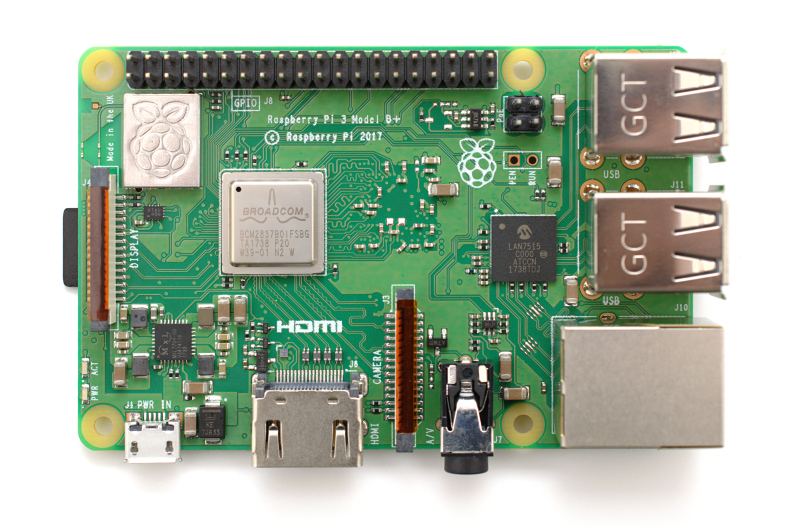
\includegraphics[height=0.1\textheight]{Figuras/Raspberry_Pi_3_B+.png}
        \caption{Raspberry Pi 3 B+ \\ (Fuente: Wikipedia\autocite{ArchivoRaspberryPi})} 
        \label{fig:RaspBerrryBPlus}
    \end{minipage}
    \hfill
    \begin{minipage}[t]{0.5\linewidth}  % <---
        \centering
        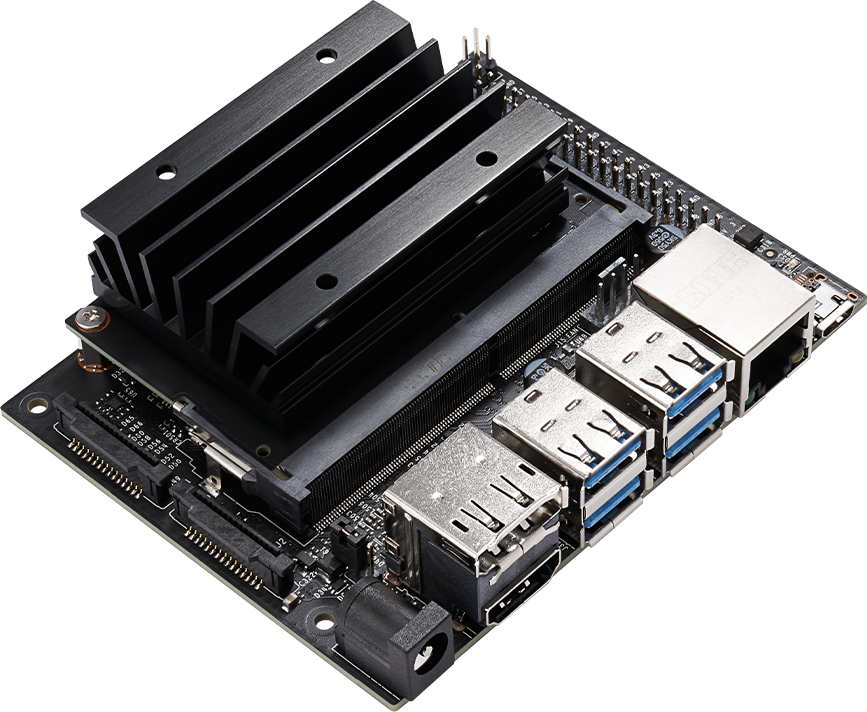
\includegraphics[height=0.1\textheight]{Figuras/nvidia_jetson_nano_2GB.png}    
        \caption{NVIDIA Jetson Nano 2GB \\ (Fuente: NVIDIA\autocite{JetsonNano})} 
        \label{fig:JetsonNano2GB}
    \end{minipage}
\end{figure}
\begin{figure}[H]
    \centering
    
\includegraphics[height=0.1\textheight]{Figuras/genius_switch.jpg}    
    \caption{Switch Genius} 
    \label{fig:Switch}
\end{figure}
\newpage

\subsubsection{Mapa de red}
Las conexiones entre los dispositivos que interactúan en la red (Raspberries y Jetson Nano) será por cable, conectando todos al mismo switch para permitir la comunicación entre ellos. A su vez, este switch se conectará al router que provee de acceso a internet, permitiendo así, que los ordenadores de la red puedan acceder a estos dispositivos y estos dispositivos puedan conectarse a internet para lo que necesiten. Todo ello queda representado en el mapa de la figura \ref{fig:MapaRed}, que sería el mapa de red físico del que parte el proyecto.
\begin{figure}[H]
    \centering
    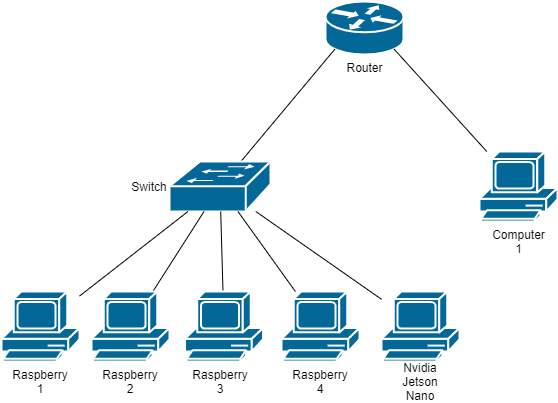
\includegraphics[width=\textwidth]{Figuras/Network_map.png}    
    \caption{Mapa de red física} 
    \label{fig:MapaRed}
\end{figure}

Esta arquitectura de red lo que permite es que desde el ordenador 1 se pueda acceder a cualquier dispositivo mediante ssh para su configuración y ejecución de experimentos. A su vez, estos dispositivos permanecen físicamente separados los unos de los otros mientras mantienen acceso a internet para realizar tareas de descarga de paquetes, actualizaciones, envío de datos, etc. En este caso, para la transferencia de archivos y ficheros se utilizará el protocolo SCP, ya que no entra dentro del alcance el desarrollo de ningún sistema de comunicación y el protocolo SCP es fácilmente combinable con el protocolo ssh.

\pagebreak

Sin embargo, desde el punto de vista de la red de FL que se quiere simular, el mapa de red incluiría los siguientes cambios:
\begin{itemize}
    \item Cada participante tendría su propia red de área local.
    \item La conexión al servidor de agregación se haría a través de internet.
    \item Los participantes no tendrían ninguna conexión ni relación entre sí.
\end{itemize}
De este modo, el mapa de la red de FL representado en el proyecto quedaría acorde a la figura \ref{fig:FLMapaRed}, aunque el mapa de red sobre el que se opere físicamente sea el de la figura \ref{fig:MapaRed}.

\begin{figure}[H]
    \centering
    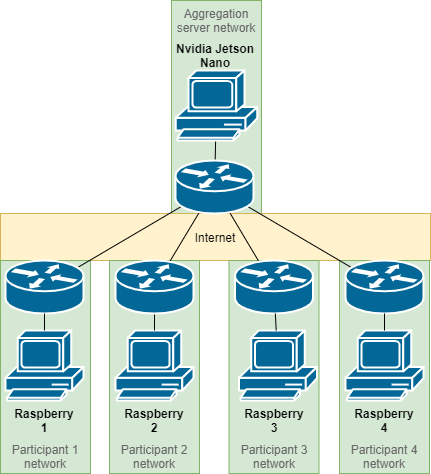
\includegraphics[width=0.8\textwidth]{Figuras/FL_network_map.png}    
    \caption{Mapa de la red de FL} 
    \label{fig:FLMapaRed}
\end{figure}

\pagebreak

\subsubsection{Montaje físico}
Una vez realizados todos los mapas y diagramas para la configuración de la red, se procedió a conectar los dispositivos acorde al mapa de red físico (fig. \ref{fig:MapaRed}). Para este montaje, se acoplaron las Raspberries que representan a los participantes en el rack mencionado en la sección de gestión de riesgos \ref{GestionRiesgos} de este mismo capítulo. Después de conectar todos los cables el montaje quedó como se puede ver en las siguientes imágenes.
\begin{figure}[H]
    \centering
    \begin{minipage}[t]{0.49\linewidth}  % <---
        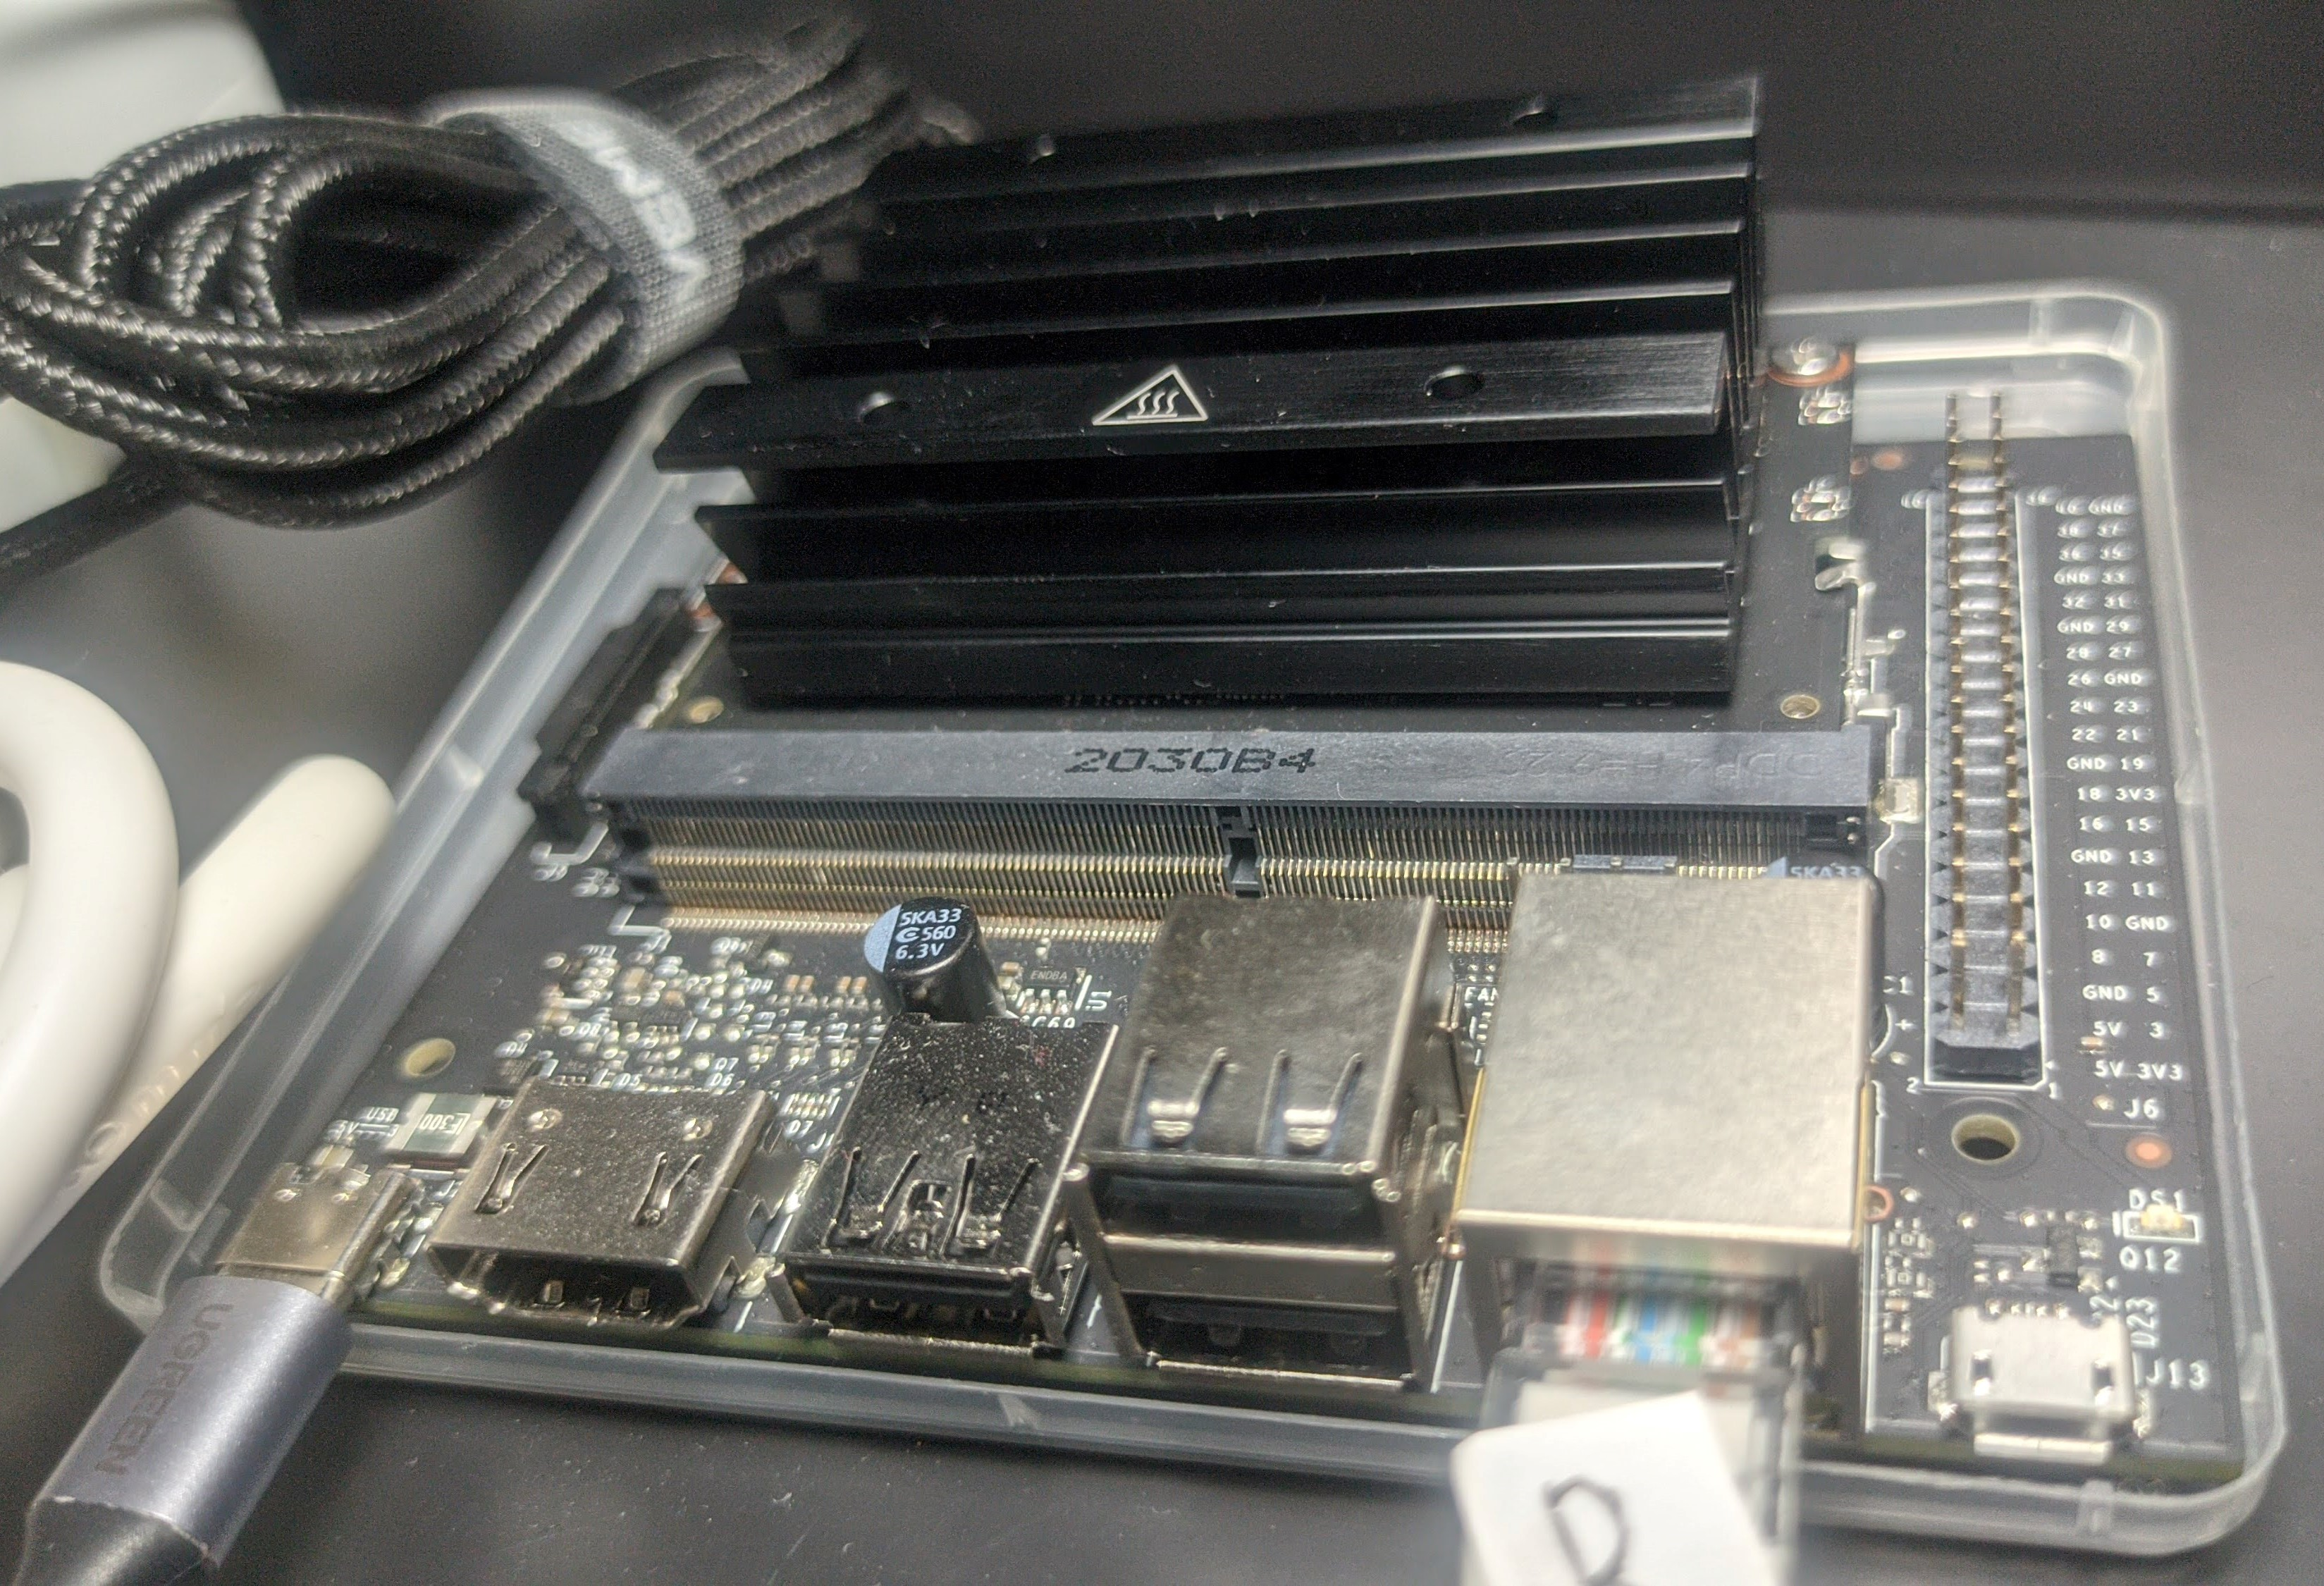
\includegraphics[height=0.2\textheight]{Figuras/jetsonnano.jpg}
        \caption{Montaje de la Jetson Nano} 
    \end{minipage}
    \hfill
    \begin{minipage}[t]{0.5\linewidth}  % <---
        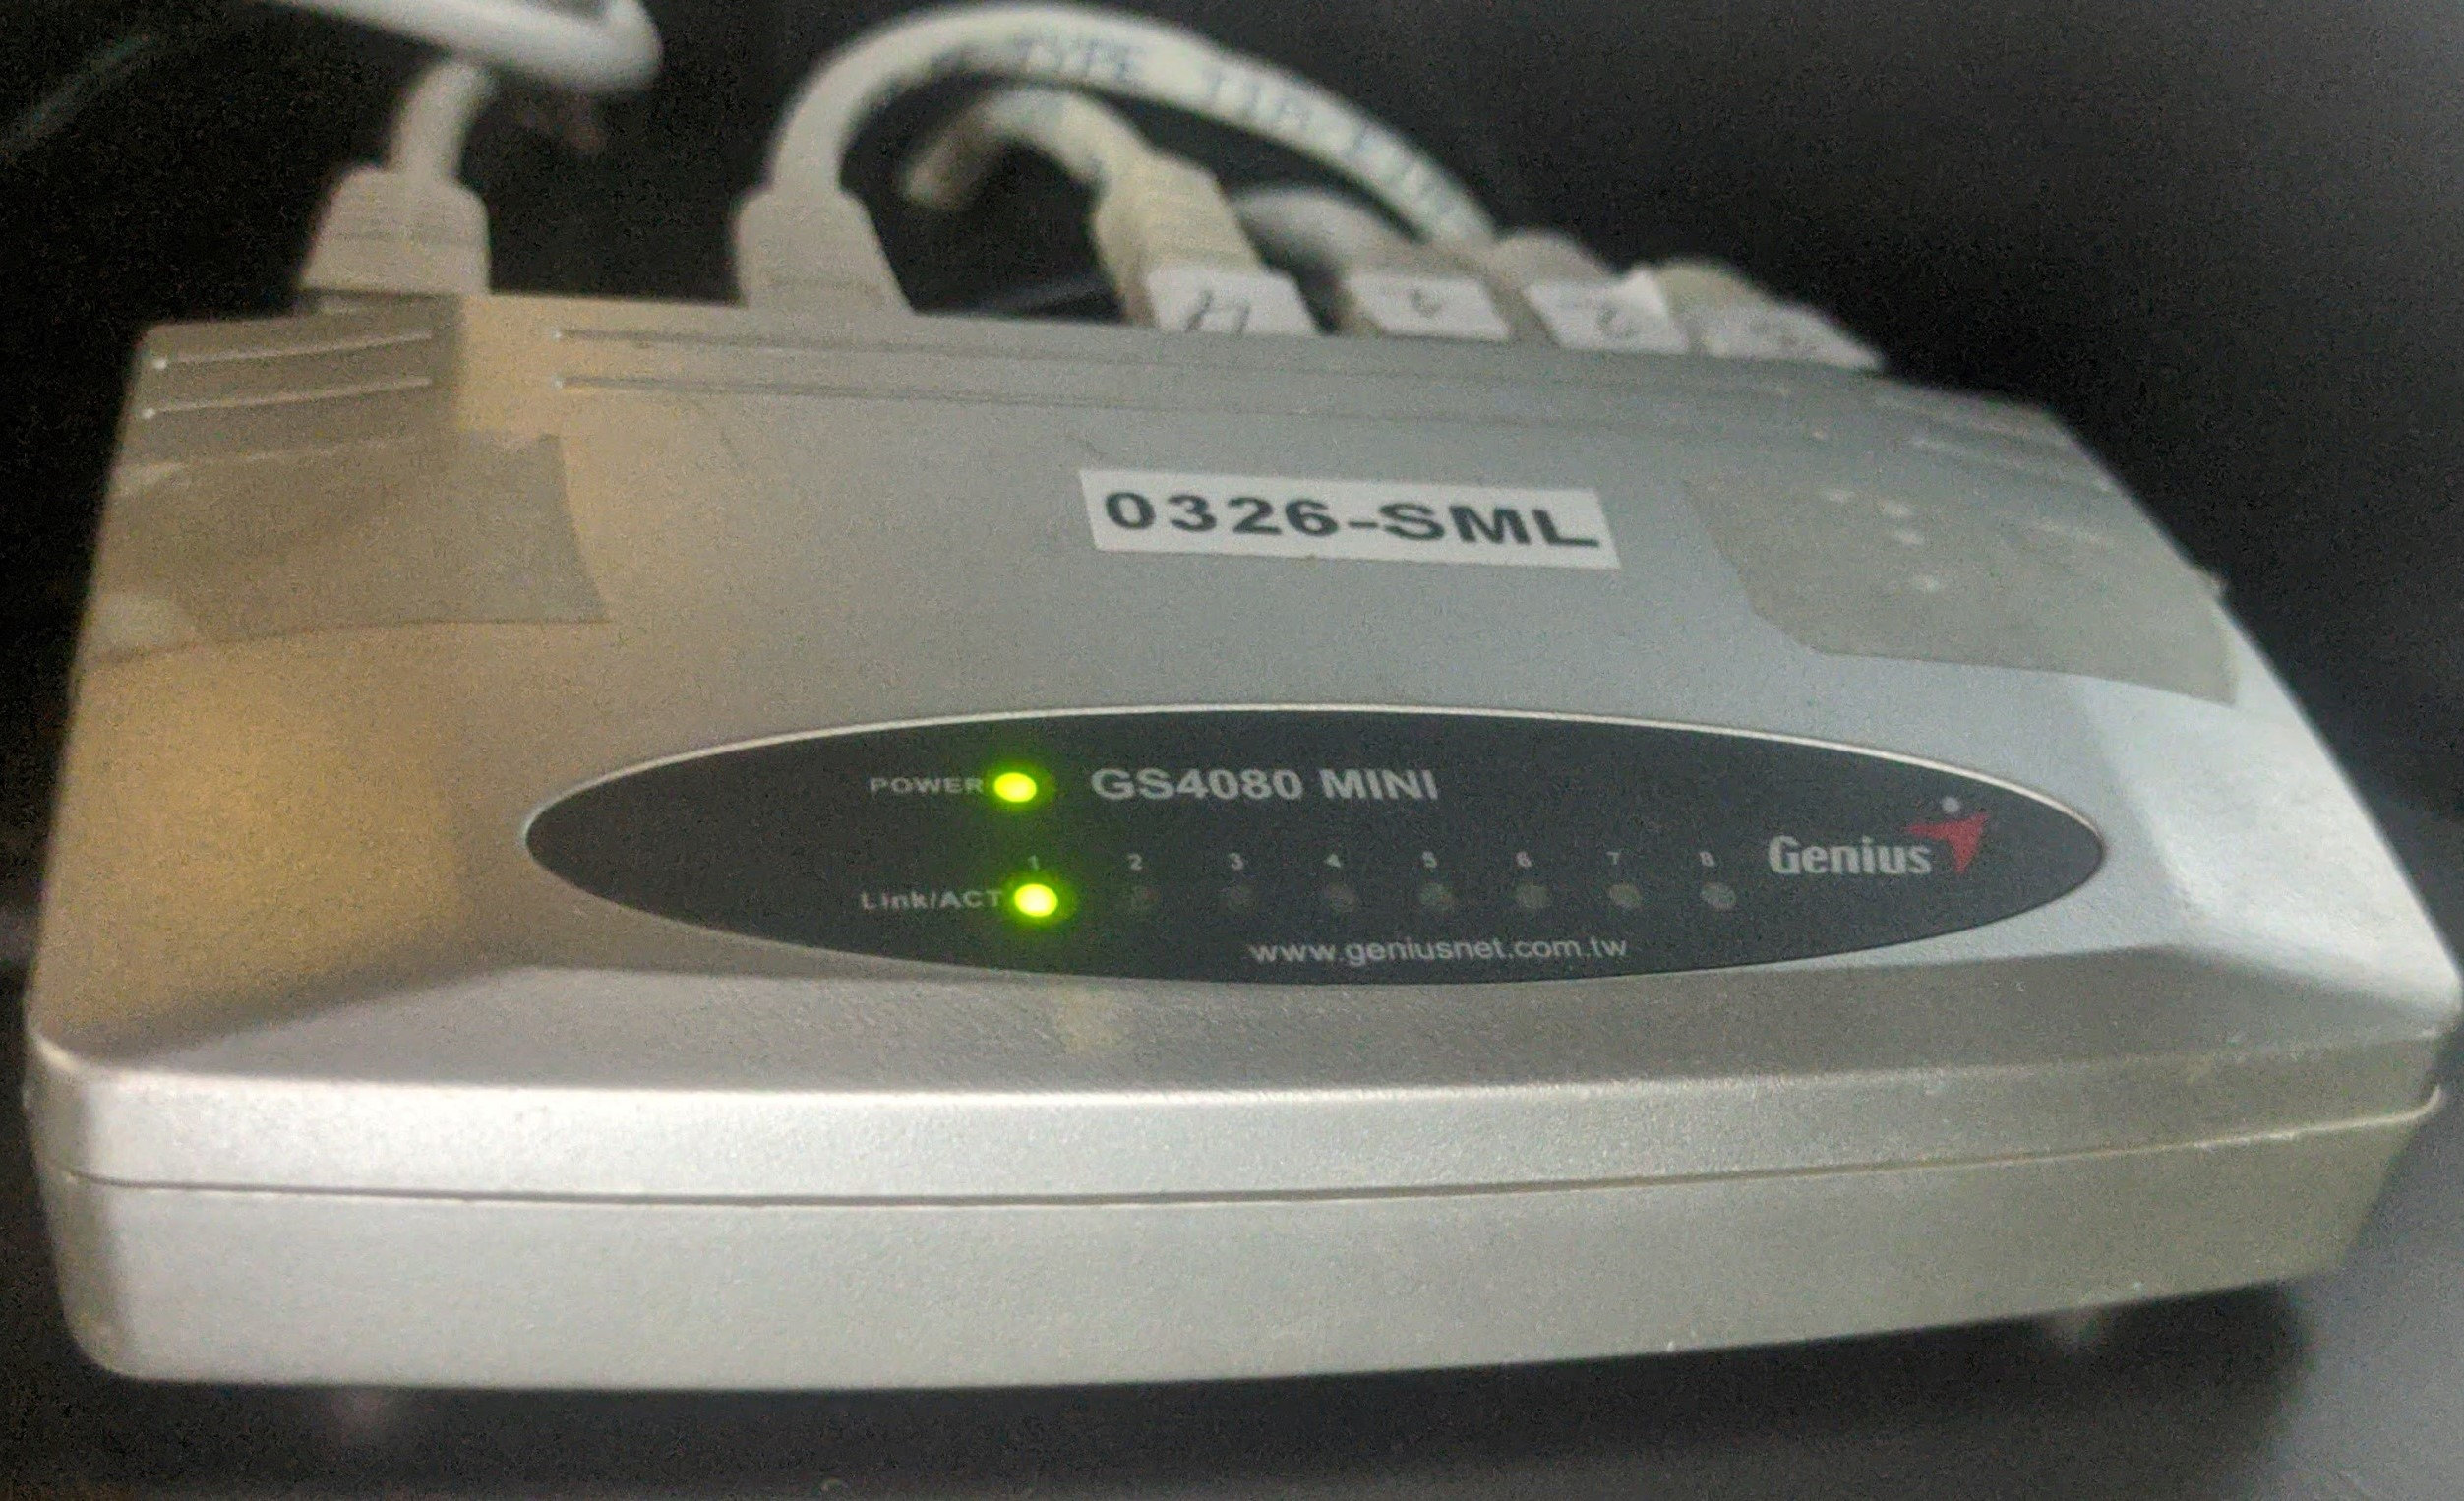
\includegraphics[height=0.2\textheight]{Figuras/switch.jpg}
        \caption{Montaje del switch} 
    \end{minipage}

    \includegraphics[width=0.75\textwidth]{Figuras/raspberrys.jpg}
    \caption{Montaje de las Raspberries}     
\end{figure}

La Jetson Nano y cada Raspberry tienen un cable ethernet conectado al switch, el cual, a su vez, cuenta con otro cable ethernet por el cual se conecta al router (no visible en las fotos).


\newpage

\subsection{Datos involucrados}
Al tratarse este proyecto de una modificación del sistema de recomendación de R.Sánchez y col., se heredarán todos los datos. Cabe mencionar que R.Sánchez y col. utilizaron información proporcionada por el proyecto Green Soul\autocite{EcoawarePersuasiveNetworked} para crear su sistema de recomendación. El proyecto Green Soul trataba de persuadir a los usuarios para que aumentase su conciencia energética y cambiaran sus hábitos de consumo, para ello, se realizaron una serie de encuestas donde se les preguntaba a los usuarios por sus datos personales y se les pedía que ordenarán en función de su criterio qué estrategias de persuasión les parecían más efectivas.
\\ \\
Por tanto, las estrategias de persuasión que se recomiendan pertenecen al ámbito de la concienciación del consumo energético, aunque podrían ser extrapolables a otros casos. De todas formas, se eludirán los detalles sobre estas estrategias ya que no son el caso de estudio y no entran en el alcance de este proyecto.
\\ \\
Teniendo en cuenta todo lo anterior, este capítulo se ha redactado para entender la gestión de los datos en este proyecto, ya que algunos son de carácter personal y es de suma importancia preservar su privacidad. Estos datos se pueden dividir en tres categorías:
\begin{itemize}
    \item \textbf{No sensibles}, la información de los elementos a recomendar, que no son ni personales ni suministrados por ninguna persona.
    \item  \textbf{Sensibles}, datos que hacen referencia a información personal o que son proporcionados por las personas involucradas en el cuestionario.
    \item \textbf{Sintéticos}, datos de usuarios generados aleatoriamente para paliar la necesidad de datos personales del modelo de consenso (sección \ref{Consenso}.Agregación de modelos por consenso).
\end{itemize} 

\subsubsection{No sensibles}
Como se ha mencionado antes, en la categoría de datos no sensibles se encuentran los datos que no son personales ni hacen referencia a ningún usuario. En esta categoría únicamente aparecen aquellos datos que hacen referencia a los elementos que se van a recomendar en el sistema y sus atributos.
\\ \\
Cada estrategia de persuasión que pueda recomendar el RS contará con hasta dos atributos, para que de esta forma, el sistema pueda conocer mejor las estrategias y realizar recomendaciones más precisas en base a esta información. En la tabla \ref{tab:EstrategiasPersuasion} se muestran las estrategias de persuasión involucradas en el RS y sus atributos.
\begin{table}[H]
    %Con esta función se inicia el entorno tabla, que se puede posicionar con respecto al texto al igual que una imagen.
    
    \begin{center}
    %Se centra la tabla.
        \begin{tabular}{|c|p{0.45\linewidth}|p{0.2\linewidth}|p{0.2\linewidth}|}
            % -------------
            \hline
            \rowcolor{Cyan} 
            % -------------
            \textbf{ID} & \textbf{Descripción} & \textbf{Atributo 1} & \textbf{Atributo 2} \\ 
            % -------------
            \hline
            \textbf{V2} &  Reconocimiento público/social de mi contribución al ahorro de energía. & Reconocimiento social & -\\
            % -------------
            \hline
            \rowcolor{GrisTabla}
            \textbf{V5} & Recibir información relacionada con la energía de una forma simple y estéticamente atractiva. & Atractivo físico & -\\
            % -------------
            \hline
            \textbf{V6} &  Recibir beneficios como recompensa por mejorar mi rendimiento energético(horarios de trabajo flexibles, saltarse ciertas tareas, etc.). & Condicionamiento & -\\
            % -------------
            \hline
            \rowcolor{GrisTabla} 
            \textbf{V7} & Recibir un reconocimiento por lograr ahorros de energía de manera colectiva yo y mi equipo. & Reciprocidad & Reconocimiento social\\
            % -------------
            \hline
            \textbf{V10} & Mis altos gerentes están comprometidos con el ahorro de energía. & Autoridad & Demostración social \\
            % -------------
            \hline
            \rowcolor{GrisTabla} 
            \textbf{V11} & Poder monitorear mi propio desempeño energético en tiempo real. & Monitorización propia. & - \\ 
            % -------------
            \hline
            \textbf{V15} &  Información sobre el efecto que mis acciones pueden tener sobre el consumo de energía. & Causa efecto & -\\
            % -------------
            \hline
            \rowcolor{GrisTabla} 
            \textbf{V17} & Evacuación comparativa de mi desempeño en el ahorro de energía respecto a usuarios parecidos a mí. & - & -\\
            % -------------
            \hline
            \textbf{V19} &  Consejos y sugerencias sobre el ahorro de energía al día o a la semana.  & Sugerencia & -\\
            % -------------
            \hline
            \rowcolor{GrisTabla} 
            \textbf{V20} &  Avances y consejos sobre las lecciones aprendidas de usuarios parecidos mí en acciones específicas de ahorro de energía. & Similaridad & -\\
            \hline

            % \rowcolor{Naranja} 
            % \textbf{V} & \textbf{elit} \\ \hline
        \end{tabular}
        \caption{\centering Estrategias de persuasión del sistema (Fuente: Elaboración propia).}
        \label{tab:EstrategiasPersuasion}
    \end{center}    
\end{table}


\subsubsection{Sensibles}
En cuanto a los datos sensibles hay que mencionar dos grupos, los datos personales de los usuarios y los rankings de los usuarios. Este primer grupo está formado por los datos personales de los usuarios participantes, que intervienen en dos puntos clave: en el entrenamiento de los modelos de IA y a la hora de agregar estos modelos. El grupo de los datos de los rankings está formado por las preferencias de los anteriores usuarios a la hora de ordenar las estrategias de persuasión, es decir, el ranking de estrategias para cada usuario.
\\ \\
Tanto los datos personales de los usuarios como los datos de los rankings de estos son necesarios para entrenar un modelo de IA. Los atributos de los usuarios, al igual que los atributos de las estrategias de persuasión, sirven para relacionar los distintos usuarios entre sí y encontrar relación entre sus diferentes atributos con el orden que le han dado a las diferentes estrategias de persuasión, de esta forma, se pueden realizar recomendaciones en base al tipo de usuario.

\paragraph{Datos de usuarios\\}
Los datos personales de los usuarios que intervienen en este proyecto son los presentes en la tabla \ref{tab:AtributosUsuarios}. Estos datos han sido transformados a objetos json para su posterior utilización, formando una lista de objetos en los que cada uno representa los datos personales de un usuario.
\begin{table}[H]
    %Con esta función se inicia el entorno tabla, que se puede posicionar con respecto al texto al igual que una imagen.
    
    \begin{center}
    %Se centra la tabla.
        \begin{tabular}{|c|c|p{0.7\linewidth}|}
            % -------------
            \hline
            \rowcolor{Cyan} 
            % -------------
            \textbf{ID} & \textbf{Nombre} & \textbf{Descripción}\\ 
            % -------------
            \hline
            \textbf{0} &  Edad & Rango de edad\\
            % -------------
            \hline
            \rowcolor{GrisTabla}
            \textbf{1} & Género & Género\\
            % -------------
            \hline
            \textbf{2} & Educación & Nivel educativo\\
            % -------------
            \hline
            \rowcolor{GrisTabla} 
            \textbf{3} & País & País de residencia\\
            % -------------
            \hline
            \textbf{4} & Cultura de trabajo & Cultura de trabajo\\
            % -------------
            \hline
            \rowcolor{GrisTabla} 
            \textbf{5} & PST & Tipo de perfil de usuario en base a los propuestos por Dan Lockton\autocite{locktonModelsUserDesigners2012} : \textit{"Pinball, Shortcut, Thought-ful"}\\ 
            % -------------
            \hline
            \textbf{6} & Barreras  & Barreras ante el cambio\\
            % -------------
            \hline
            \rowcolor{GrisTabla} 
            \textbf{7} & Intenciones & Intenciones ante el cambio\\
            % -------------
            \hline
            \textbf{8} & Confianza  & Confianza ante el cambio\\
            % -------------
            \hline

            % \rowcolor{Naranja} 
            % \textbf{V} & \textbf{elit} \\ \hline
        \end{tabular}
        \caption{\centering Atributos de los usuarios que participan en el sistema (Fuente: Elaboración propia).}
        \label{tab:AtributosUsuarios}
    \end{center}    
\end{table}
\paragraph{Rankings\\}
Los usuarios, a parte de introducir sus datos personales anteriores, también introducen el orden de las estrategias de persuasión en base a la relevancia que consideran que tienen. Este ranking de estrategia es recogido y transformado a formato json formando una lista de objetos json en la que cada objeto representa los datos de la tabla \ref{tab:RankingUsuario}.
\begin{table}[H]
    \begin{center}
    %Se centra la tabla.
        \begin{tabular}{|c|p{0.7\linewidth}|}
            % -------------
            \hline
            \rowcolor{Cyan} 
            % -------------
            \textbf{Nombre} & \textbf{Descripción}\\ 
            % -------------
            \hline
            \textbf{User ID}  & Identificador único del usuario\\
            % -------------
            \hline
            \rowcolor{GrisTabla}
            \textbf{Item ID}  & Identificador único de la estrategia de persuasión\\
            % -------------
            \hline
            \textbf{Ranking} & Valor en el ranking de la estrategia de persuasión\\
            % -------------
            \hline
            % \rowcolor{Naranja} 
            % \textbf{V} & \textbf{elit} \\ \hline
        \end{tabular}
        \caption{\centering Elementos de la estructura de los datos del ranking  (Fuente: Elaboración propia).}
        \label{tab:RankingUsuario}
    \end{center}    
\end{table}


\subsubsection{Sintéticos}
En cuanto a los datos sintéticos, se debe tener en cuenta que los datos sensibles han sido directamente suministrados por los usuarios, por lo cual, es técnicamente imposible acceder a ellos desde el servidor de agregación, ya que sería una evidente violación de la privacidad de los usuarios. Esto genera un gran problema debido a que el propio modelo de consenso, explicado en la sección \ref{Consenso}, requiere de datos de usuarios para funcionar.
\\ \\
La forma de abordar el problema de la necesidad de datos es mediante la creación de usuarios sintéticos, como se explica en la subsección \ref{Consenso:Usuarios_Sinteticos}. Estos usuarios sintéticos tendrán los mismos atributos que los usuarios normales (tabla \ref{tab:AtributosUsuarios}), tendrán que clasificar las mismas estrategias de persuasión (tabla \ref{tab:EstrategiasPersuasion}) y el ranking se gestionará de la misma forma (tabla \ref{tab:RankingUsuario}).


\newpage

\subsection{Protocolo de Federated Learning}\label{Protocolo}
El protocolo de Federated Learning que se va a reproducir en este proyecto es una adaptación de lo que proponen K. Bonawitz y col. \autocite{bonawitzFederatedLearningScale2019a}. En este protocolo se definen tres fases importantes, la selección de participantes, la configuración del mecanismo de agregación y el envío reporte de cada participante.
\\\\
Para este caso se han introducido leves cambios en este protocolo que se irán explicando en las sucesivas partes del mismo.  

\subsubsection{Selección de participantes}
La selección de participantes al tratarse de un caso de estudio concreto no se limita ni se controla de ninguna forma, simplemente se ha implementado una red en la que participan cuatro dispositivos diferentes.

\subsubsection{Intercambio de claves}
El intercambio de claves es una de las novedades introducidas sobre el protocolo previamente mencionado, en este paso, el objetivo es que los diferentes dispositivos de la red compartan sus claves públicas para poder asegurar la privacidad de la red, imagen \ref{fig:PublicKeyShare}. 
\\ \\
La utilización de estas claves públicas y su función están definidas en el apartado de securización de las comunicaciones \ref{SegCom}.
\begin{figure}[H]
    \centering
    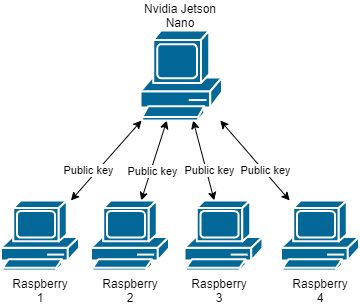
\includegraphics[width=0.5\textwidth]{Figuras/Network_public_key.png}    
    \caption{Intercambio de claves públicas entre los participantes} 
    \label{fig:PublicKeyShare}
\end{figure}

\subsubsection{Entrenamiento}
El entrenamiento es algo que en el protocolo se omite pero que es importante mencionar. Este proceso se lleva a cabo en el dispositivo del participante y conlleva dos tareas:
\begin{itemize}
    \item En primer lugar este participante crea su modelo de IA, lo entrena con los datos que él elija y lo almacena.
    \item En segundo lugar este modelo es cifrado y enviado al servidor. El proceso de cifrado se puede observar en el diagrama \ref{fig:Flow_Encryption} de la sección de securización de las comunicaciones \ref{SegCom}.
\end{itemize} 
\begin{figure}[H]
    \centering
    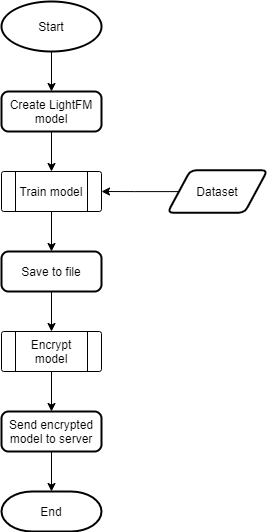
\includegraphics[height=0.6\textheight]{Figuras/flowchart_train.png}    
    \caption{Intercambio de claves públicas entre los participantes} 
    \label{fig:Entrenamiento}
\end{figure}

\subsubsection{Comunicación con el servidor}
La comunicación con el servidor es un proceso crucial en el que se debe asegurar que los modelos de los participantes lleguen sin modificaciones y sin ser interceptados por ningún atacante. Para detallar este proceso se ha elaborado una sección donde se explican más a fondo los pasos llevados para conseguir que las comunicaciones sean seguras, sección \ref{SegCom}.
\\ \\
Debido a este protocolo de seguridad, los participantes deberán enviar tanto los modelos cifrados como las claves cifradas, como se puede observar en las siguientes imágenes.

\begin{figure}[H]
    \begin{minipage}[t]{0.45\linewidth}  % <---
        \centering
        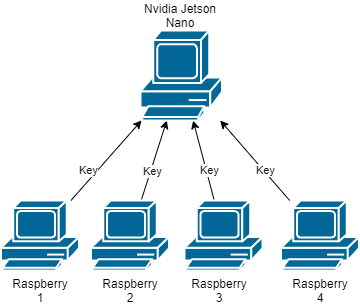
\includegraphics[width=\textwidth]{Figuras/Network_participant_encrypted_key.png}
        \caption{Envío de la clave de cifrado del modelo al servidor de agregación} 
    \end{minipage}
    \hfill
    \begin{minipage}[t]{0.45\linewidth}  % <---
        \centering
        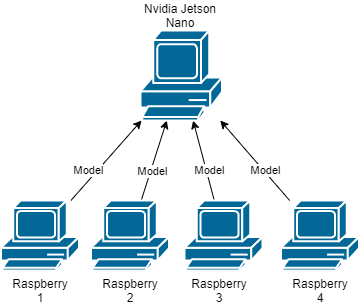
\includegraphics[width=\textwidth]{Figuras/Network_participant_encrypted_model.png}    
        \caption{Envío del modelo cifrado al servidor de agregación} 
    \end{minipage}
\end{figure}

\subsubsection{Agregación de los modelos}
En este proceso, como tal, no va a ocurrir una agregación de modelos, sino más bien una compartición de conocimiento de forma indirecta mediante el modelo de consenso. Este sistema está explicado con detalle en la sección \ref{Consenso} de este capítulo.
\\ \\
De todas formas, para verlo de una forma más sencilla, se puede observar el siguiente diagrama \ref{fig:Flow_Agregation} en el cual se muestra el flujo de los datos y de los modelos para ser agregados. El proceso que recorre este diagrama puede ser dividido en 4 partes:
\begin{itemize}
    \item Se reciben los modelos de los participantes (en este caso 4), se descifran siguiendo el diagrama \ref{fig:Flow_Decryption} (explicado con detalle en en la sección de securización de las comunicaciones \ref{SegCom}) y se guardan los modelos para su posterior utilización.
    \item Una vez se cuente con los modelos descifrados, se generan los usuarios sintéticos, después, con el modelo de cada participante se realiza la predicción del ranking para estos usuarios y se almacena para su posterior utilización. 
    \item Mediante el modelo de consenso explicado en el apartado \ref{Consenso} estas predicciones son convertidas a una única predicción por usuario sintético generado. Después, la información se almacena para su uso final.
    \item Por último, se coge toda la información de los usuarios sintéticos y los rankings consensuados para reentrenar el modelo de cada participante. 
\end{itemize}
\begin{figure}[H]
    \centering
    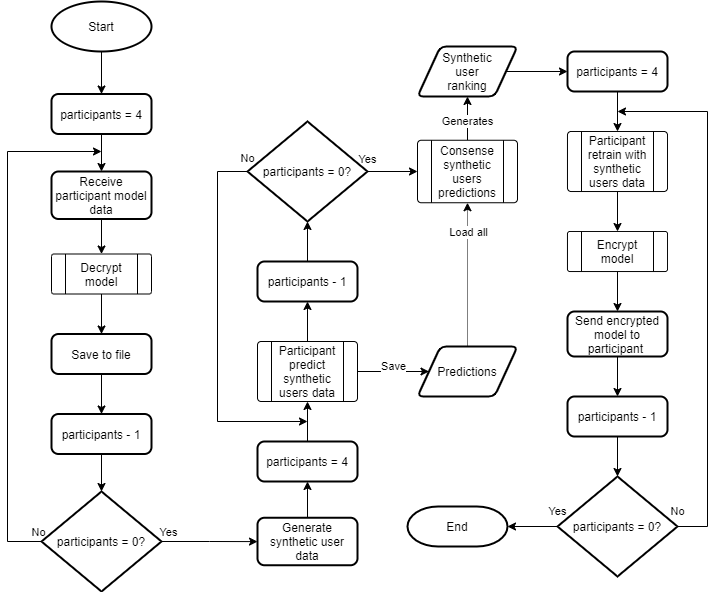
\includegraphics[width=\textwidth]{Figuras/flowchart_agregation.png}    
    \caption{Diagrama del flujo de reentrenado de los modelos} 
    \label{fig:Flow_Agregation}
\end{figure}
\newpage
\subsubsection{Comunicación con los participantes}
La comunicación con los participantes se realiza de la misma forma que los participantes se comunican con el servidor, la única diferencia es que el receptor en este caso son los participantes.
\begin{figure}[H]
    \begin{minipage}[t]{0.45\linewidth}  % <---
        \centering
        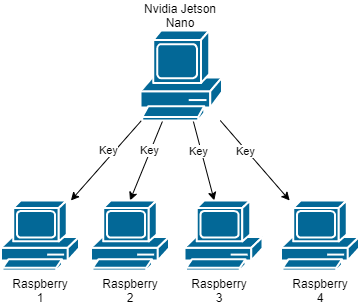
\includegraphics[width=\textwidth]{Figuras/Network_node_encrypted_key.png}
        \caption{Envío de la clave de cifrado del modelo de cada participante a cada participante} 
    \end{minipage}
    \hfill
    \begin{minipage}[t]{0.45\linewidth}  % <---
        \centering
        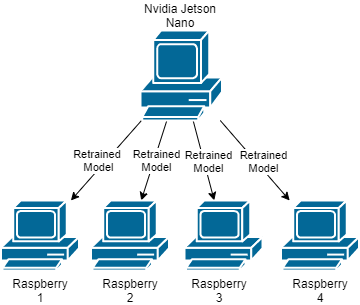
\includegraphics[width=\textwidth]{Figuras/Network_node_encrypted_model.png}    
        \caption{Envío de cada modelo cifrado a su correspondiente dueño} 
    \end{minipage}
\end{figure}
\subsubsection{Comparación de modelos}
En el momento que el modelo llega al participante este tiene que valorar si realmente le supone una mejora o no, para ello como puede verse en el diagrama \ref{fig:Flow_Compare}, existen varias fases a llevar a cabo.

En primer lugar, al igual que como con el servidor de agregación, se debe descifrar el modelo recibido. Después, compararlo con el modelo del participante, esto se puede hacer tratando de analizar la precisión de las predicciones para varios subconjuntos de datos de test con los que cuente el dispositivo. En resumen, predecir para los usuarios existentes de su ranking con los dos modelos y quedarse con el modelo que más acierte.

\begin{figure}[H]
    \centering
    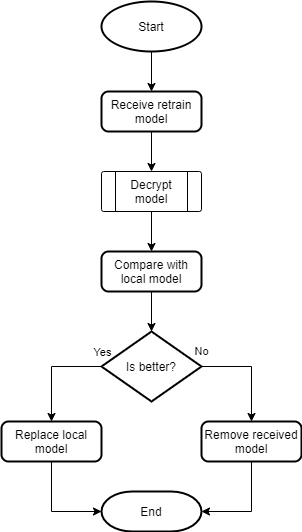
\includegraphics[height=0.6\textheight]{Figuras/flowchart_compare.png}    
    \caption{Diagrama del flujo de la comparación de los modelos} 
    \label{fig:Flow_Compare}
\end{figure}


\newpage

\subsection{Securización de las comunicaciones}
Para preservar la seguridad y privacidad en el protocolo de aprendizaje federado propuesto es imprescindible securizar las comunicaciones. Para securizarlas se han llevado a cabo dos acciones clave, la primera en lo que concierne al protocolo de comunicación y la segunda en cuanto al cifrado de la comunicación.

\subsubsection{Protocolo de comunicación}
En cuanto al protocolo de comunicación se ha optado por la utilización del protocolo SCP (Secure Copy Protocol), conocido en español como protocolo de copia segura. Este protocolo requiere del protocolo SSH (Secure Shell), conocido en español como terminal seguro.
\\ \\
El protocolo SSH permite el acceso remoto a un servidor o dispositivo por un canal seguro a través de una clave. Además, el protocolo usa técnicas de cifrado que impiden que la información que viaje en la red lo haga de forma legible. El protocolo SCP permite la transferencia de archivos entre dispositivos de la red usando el protocolo SSH como base.

\subsubsection{Cifrado de la comunicación}
Aunque las comunicaciones en el protocolo SCP y SSH vayan cifradas son susceptibles de ser atacadas. Para mejorar este aspecto se ha realizado un sistema de cifrado de los modelos que viajen por la red para preservar la privacidad y seguridad de los participantes.
\\ \\ 
Para esta labor se han utilizado el método criptográfico de criptografía híbrida, que usa tanto la criptografía simétrica como asimétrica.

\paragraph{Cifrado simétrico} 
El cifrado simétrico es aquel sistema de cifrado en el que la misma clave sirve para cifrar como para descifrar el mensaje. 
\\ \\
El problema de este sistema es que toda la seguridad reside en la clave empleada en el cifrado. Esto es un gran impedimento a la hora de gestionar comunicaciones debido al cómo gestionar el envío de esta clave, ya que si no se hace por un canal seguro el mensaje sera fácilmente descifrable.
\\ \\
Por otro lado, este sistema cuenta con dos grandes ventajas, es sencillo, es rápido y requiere menos recursos para llevarlo a cabo.

\paragraph{Cifrado asimétrico}
El cifrado asimétrico es aquel sistema de cifrado que consta de dos claves criptográficas, una pública y una privada. La clave pública es utilizada para cifrar el mensaje mientras que la privada es utilizada para descifrarlo. 
\\ \\
Este sistema cuenta con tres grandes desventajas que impiden su uso en exclusivo o su uso con grandes volúmenes de información a cifrar. 
\begin{itemize}
    \item Se necesita más procesado de computo para generar la clave.
    \item Las claves asimétricas son mucho más grandes que las simétricas.
    \item El mensaje cifrado ocupa más espacio que el original.
\end{itemize}

Debido a que los dispositivos con los que se cuenta no tienen una gran capacidad de computo no se podría establecer un tamaño de clave lo suficientemente grande como para poder cifrar el modelo de inteligencia artificial completo. Este modelo pesa al rededor de los 7Kb y para cifrarlo con este sistema habría que generar una clave del mismo tamaño mayor.
\\ \\
Sin embargo, este sistema al constar de dos claves independientes es más sencillo salvaguardar la privacidad y seguridad de los integrantes.

\paragraph{Cifrado híbrido}
Teniendo en cuenta los anteriores dos tipos de cifrado se decidió utilizar el sistema híbrido para obtener los resultados más óptimos, protegiendo la privacidad y pudiendo realizar las tareas de cifrado desde dispositivos con menor capacidad computacional.
\\ \\ 
El proceso de cifrado se ha realizado de acorde al diagrama de flujo representado en la figura \ref{fig:Flow_Encryption}. En este diagrama se pueden observar los pasos que se han realizado para la encriptación de la información, en primer lugar el modelo de LightFM se convertió a bytes y se comprimió para reducir el volumen de datos a enviar por la red, pudiendo agilizar así las comunicaciones. Después se cifró simétricamente, generando una clave y un mensaje cifrado. Por un lado este mensaje cifrado sería comprimido y se guardaría en un fichero para su posterior envío. Por otro lado, la clave de cifrado simétrica se encriptó asimetricamente con la clave pública del receptor del mensaje, dando como resultado una clave de cifrado simétrico cifrada asimetricamente. Esta clave sería guardada en un fichero para ser enviada al igual que el mensaje.
\begin{figure}[H]
    \centering
    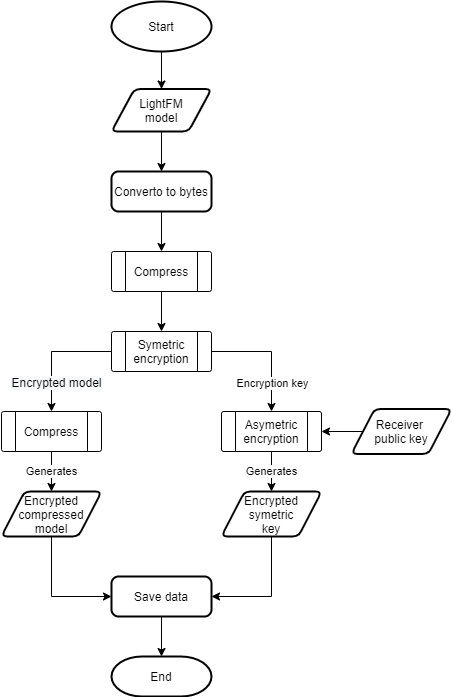
\includegraphics[height=0.6\textheight]{Figuras/flowchart_encryption.png}    
    \caption{Diagrama de flujo del proceso de cifrado} 
    \label{fig:Flow_Encryption}
\end{figure}


\subsubsection{Descifrado del mensaje}
El descifrado del mensaje es el proceso inverso al cifrado de la figura \ref{fig:Flow_Encryption}. Para ello, en un primer momento se reciben tanto el modelo cifrado simétricamente como la clave del modelo cifrada asimétricamente. En primer lugar, la clave que se ha recibido se descifra asimétricamente con la clave privada propia, ya que esta solo es descifrable por el receptor. Una vez descifrada la clave, se descomprime el modelo y se descifra con esta. Por último, el resultado es descomprimido y convertido a objeto LightFM para su posterior utilización. 
\begin{figure}[H]
    \centering
    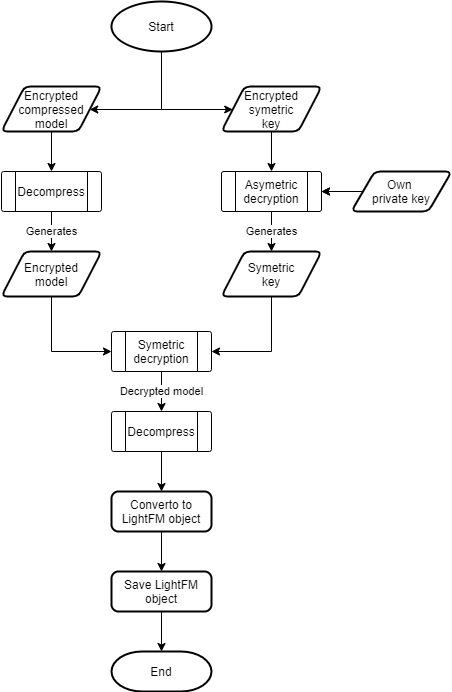
\includegraphics[height=0.6\textheight]{Figuras/flowchart_decryption.png}    
    \caption{Diagrama de flujo del proceso de descifrado} 
    \label{fig:Flow_Decryption}
\end{figure}

\newpage


\subsection{Agregación de modelos por consenso}\label{Consenso}
A la hora de agregar los diferentes modelos de los participantes se estudiaron los distintos algoritmos de los sistemas de FL, pero todos tenían algo en común, accedían a los datos del modelo. Aunque estos datos de los modelos sean meras matrices y números, el objetivo de este proyecto era no acceder en ningún momento a la información presente en ellos, por lo que se buscó otra solución.
\\ \\
La solución llegó con un cambio de enfoque. Se dejó de combinar los distintos modelos para crear uno global y se pasó a compartir únicamente sus formas de operar. Esto se debe a que en la agregación de modelos se suelen ensamblar los modelos de los distintos participantes. Es decir, se combinan los modelos o se extraen de cada modelo ciertos parámetros para crear uno general. El problema presente en estos enfoques tradicionales es que se accede a la información de los modelos de forma directa, objetivo principal a evitar en este proyecto.
\\ \\
El enfoque de compartir la forma de operar de los distintos modelos de IA se empezó a explorar mediante la generación de usuarios sintéticos, para los cuales, el modelo de cada participante de la red de FL debería predecir su ranking. Cuando cada participante predice el ranking para cada usuario sintético están demostrando cómo actuarían ante ciertas entradas de datos, por lo que si se compartiera este conocimiento, los participantes se verían beneficiados de las formas de operar de otros participantes.
\\ \\
El problema es que, desde un punto de vista objetivo, puede que algunas formas de operar no sean del todo \textit{precisas}, por lo que no se debería compartir los rankings predichos por todos los modelos sin ningún tipo de filtrado. Para realizar este filtrado y con el objetivo de llegar a un punto intermedio se creó el modelo de consenso, en el cual las predicciones que da cada modelo para los usuarios sintéticos se combinan de forma que todos los modelos lleguen a un acuerdo para el ranking de cada usuario. 
\\ \\
Este modelo de consenso se explicará en los siguientes apartados, donde se enseñará cómo se generan los datos sintéticos, como se generan los rankings, las explicaciones matemáticas del consenso y el proceso de reentrenado de los modelos.

\subsubsection{Generar datos personales sintéticos}\label{Consenso:Usuarios_Sinteticos}
Uno de los elementos imprescindibles para poner en práctica el sistema de agregación por consenso, es la necesidad de datos de usuarios, que con el objetivo de evitar cualquier violación de privacidad serán creados en el servidor, siendo de ahora en adelante denominados como usuarios sintéticos.
\\ \\
Estos usuarios sintéticos tendrán los mismos atributos que cualquier usuario del sistema, es decir, contarán con todos los atributos presentes en la tabla \ref{tab:AtributosUsuarios}. Como ya se ha dicho antes, el proceso de creación de estos datos es crucial para el correcto funcionamiento del sistema, ya que si los usuarios generados fueran de un perfil concreto, el aprendizaje no sería favorable para todos los participantes de la red, puesto que lo más seguro es que únicamente el participante con más usuarios de este perfil sea beneficiado, mientras que para los demás participantes, supondrá una pérdida de precisión por el ruido introducido en su modelo. Es por eso que se ha tomado la decisión de generarlos aleatoriamente, evitando así estancarse en perfiles concretos y tratando de favorecer a todos los participantes. 
\subsubsection{Generar ranking de los usuarios}
Los datos de los usuarios sintéticos por sí solos no son suficientes ni para entrenar ni para mejorar ningún modelo de IA, hace falta saber el ranking que estos usuarios sintéticos darían a las diferentes estrategias de persuasión, tabla \ref{tab:EstrategiasPersuasion}. 
\\ \\
Esta cuestión no puede ser abordada aleatoriamente como la anterior, ya que cada usuario ordena en base a su opinión y sus preferencias las estrategias de persuasión, por lo cual, de hacerlo aleatoriamente, se distorsionaría la realidad y no sería representativo. Además, si este ranking se generase aleatoriamente y se compartiera con los participantes de la red, distorsionaría por completo sus modelos, lo que llevaría a una pérdida inmensa de precisión. 
\\ \\
Es debido a esta problemática que se ha creado el método de consenso. Este método trata de representar la \textit{``opinión''} de cada participante de la red mediante la estimación del ranking para cada usuario sintético. Todas estas \textit{``opiniones''} serán puestas en común mediante el algoritmo de consenso, lo que dará como resultado un ranking por usuario sintético, que será usado con los datos del usuario sintético para reentrenar los modelos.
\newpage
\subsubsection{Consenso}
El proceso de consenso comienza con la ya mencionada creación de usuarios sintéticos aleatoriamente, pero la generación del ranking de estos se lleva a cabo de la siguiente manera.

\paragraph{Estructuras básicas} En primer lugar hay que definir la lista de las estrategias \textit{E} a ser ordenadas por los modelos \textit{m} de los participantes, que en este caso serán las mismas que las de la tabla \ref{tab:EstrategiasPersuasion}. Estas estrategias serán representadas como \textit{e$_{j}$}, siendo \textit{j} la cantidad de estrategias de la lista \textit{E} y \textit{e$_{j}$} la estrategia final de esta lista. 
\[
    \textit{E} = \begin{bmatrix} \textit{e$_{1}$} & \textit{e$_{2}$} & \textit{e$_{3}$} & \textit{e$_{4}$} & \cdots & \textit{e$_{j}$} \end{bmatrix}
\]
A la hora de crear una predicción de ranking, denotada \textit{r}, para las estrategias \textit{e$_j$} $\in$ \textit{E} se representará cada estrategia con un valor \textit{a}, siendo \textit{a} el puesto de la estrategia de persuasión en el ranking. Por lo cual, \textit{a} ha de ser siempre menor o igual que el número total de estrategias y mayor que cero, para así, mantenerse dentro del rango de \textit{E} (0$<$
\textit{a }$\leq$\textit{ j}), puesto que cada predicción \textit{r} no es más que una mera valoración de un usuario de las \textit{j} estrategias \textit{e} de la lista \textit{E}.
\[
    \textit{r} = \begin{bmatrix} \textit{a$_{1}$} & \textit{a$_{2}$} & \textit{a$_{3}$} & \textit{a$_{4}$} & \cdots & \textit{a$_{j}$} \end{bmatrix}
\]
De esta forma, se puede afirmar que el primer elemento del ranking tendrá el valor 1 y el último el valor \textit{j}, quedándose las demás estrategias con el resto de los puestos en ese rango. Lo que en un conjunto de 10 estrategias se traduce en que la mejor estrategia obtendría el valor 1 y la peor el valor 10.
\\ \\
Sin embargo, cuando se trata de realizar varias predicciones se simboliza como una matriz \textit{R}, donde cada predicción es representada por \textit{r$_{i}$}, en el que \textit{r} denota la predicción del ranking  e \textit{i} denota la cantidad de predicciones \textit{r} realizadas.
\[  
    \textit{R} = 
    \begin{pmatrix}
        \textit{r$_{1}$}  \\ 
        \textit{r$_{2}$}  \\ 
        \vdots  \\ 
        \textit{r$_{i}$}
    \end{pmatrix} 
    =
    \begin{pmatrix}
        a_{11}  &  a_{12}  &  \cdots   & a_{1j} \\ 
        a_{21}  &  a_{22}  &  \cdots   & a_{2j}\\ 
        \vdots  &  \vdots  &  \ddots & \vdots  \\ 
        a_{i1}  &  a_{i2}  &  \cdots   & a_{ij}
    \end{pmatrix}
\]
\newpage
\paragraph{Predicción} Una vez entendidas las estructuras básicas que se utilizarán en el método de consenso, este apartado presentará su aplicación, ya que en este apartado se crearán las predicciones que serán consensuadas a posteriori para generar los datos de reentrenamiento.
\\ \\
Se debe tener en cuenta que las operaciones anteriores cambian por completo cuando se realizan predicciones para un conjunto \textit{U} de usuarios, y si además, estas predicciones se hacen con los diferentes modelos \textit{m} de los participantes, las operaciones se complican bastante. 
\\ \\
En primer lugar, se ha de especificar que el conjunto de usuarios \textit{U} estará formado por los \textit{k} identificadores de los usuarios, representados como \textit{u$_{k}$}. Este conjunto de identificadores se crea cuando se generan los datos personales sintéticos y recoge todos los identificadores de todos los usuarios generados aleatoriamente.
\[
        \textit{U} = \begin{bmatrix} \textit{u$_{1}$} & \textit{u$_{2}$} & \textit{u$_{3}$} & \textit{u$_{4}$} & \cdots & \textit{u$_{k}$} \end{bmatrix}
\]
Para realizar las distintas predicciones con el modelo \textit{m} de cada participante de la red de FL, hay que tener en cuenta que las predicciones \textit{R} pertenecerán al modelo \textit{m}, por lo que se denotará a partir de ahora como \textit{R$_{m}$}. Además, esta matriz de predicciones \textit{R$_{m}$} estará formada por las distintas predicciones para los distintos usuarios \textit{u}, lo que será representado como \textit{r$_{u}$}.
\[  \textit{R$_{m}$} = 
    \begin{pmatrix}
        \textit{r$_{1}$}  \\ 
        \textit{r$_{2}$}  \\ 
        \vdots  \\ 
        \textit{r$_{u}$}
    \end{pmatrix} 
    =
    \begin{pmatrix}
        a_{11}  &  a_{12}  &  \cdots   & a_{1j} \\ 
        a_{21}  &  a_{22}  &  \cdots   & a_{2j}\\ 
        \vdots  &  \vdots  &  \ddots & \vdots  \\ 
        a_{u1}  &  a_{u2}  &  \cdots   & a_{uj}
    \end{pmatrix}
\]
\newpage
\paragraph{Redistribución de las predicciones}
Las predicciones realizadas con cada modelo \textit{m} sobre el conjunto de usuarios \textit{U} puede ser interpretada de diferente forma. En un principio se entiende que cada modelo \textit{m} genera una predicción \textit{R} para cada uno de los \textit{u} usuarios generados, pero del mismo modo, se puede entender que cada usuario \textit{u} obtiene una predicción \textit{r} por cada modelo \textit{m} y que con la unión de todas las predicciones \textit{r} de todos los modelos \textit{m} para este mismo usuario \textit{u} se puede construir una matriz \textit{R}. 
\\ \\
Para entender lo anterior con más facilidad se ha de comprender que ya no solo se cuenta con una matriz de predicciones \textit{R}, sino que se cuenta con una matriz \textit{P} con \textit{m} matrices de predicciones \textit{R}, denotada como \textit{P$_{m}$}. Esta matriz representa todas las predicciones \textit{R} realizadas por cada modelo \textit{m} participante en la red de FL para un mismo conjunto de usuarios \textit{U}.
\[
    \textit{P$_{m}$}=
    \begin{pmatrix}
        \begin{pmatrix}
            a_{11}  &  a_{12}  &  \cdots   & a_{1j} \\ 
            a_{21}  &  a_{22}  &  \cdots   & a_{2j}\\ 
            \vdots  &  \vdots  &  \ddots & \vdots  \\ 
            a_{u1}  &  a_{u2}  &  \cdots   & a_{uj}
        \end{pmatrix}_{\textit{1}}
        & 
        \cdots 
        &
        \begin{pmatrix}
            a_{11}  &  a_{12}  &  \cdots   & a_{1j} \\ 
            a_{21}  &  a_{22}  &  \cdots   & a_{2j}\\ 
            \vdots  &  \vdots  &  \ddots & \vdots  \\ 
            a_{u1}  &  a_{u2}  &  \cdots   & a_{uj}
        \end{pmatrix}_{\textit{m}}
    \end{pmatrix}
\]
Teniendo en cuenta esta estructura de datos, la separación de los usuarios ha de hacerse tomando cada predicción \textit{r$_{u}$} de cada participante de forma separada, uniendo las que corresponden al mismo usuario \textit{u} en una nueva matriz de predicciones \textit{R}, que al pertenecer al usuario \textit{u} será denotada como \textit{R$_{u}$}. Cada predicción \textit{r} de \textit{R$_{u}$} es extraída de la predicción \textit{r$_{u}$} de la matriz de predicciones de cada modelo \textit{R$_{m}$}. Además, todas las matrices de predicción \textit{R} de todos los usuarios \textit{u} serán agrupadas bajo el termino \textit{P$_{u}$}. De esta, forma puede afirmarse que \textit{P$_{u}$} está formada por las distintas predicciones \textit{R$_{u}$}, las cuales a su vez están formadas por las distintas predicciones \textit{r$_{u}$} extraídas de \textit{R$_{m}$}.

\[  \textit{R$_{m}$} = 
    \begin{pmatrix}
        a_{11}  &  a_{12}  &  \cdots   & a_{1j} \\ 
        a_{21}  &  a_{22}  &  \cdots   & a_{2j}\\ 
        \vdots  &  \vdots  &  \ddots & \vdots  \\ 
        a_{u1}  &  a_{u2}  &  \cdots   & a_{uj}
    \end{pmatrix}
    \equiv
    \begin{pmatrix}
        \begin{pmatrix} a_{1}  &  a_{2}  &  \cdots   & a_{j} \end{pmatrix}_{1} \\ 
        \begin{pmatrix} a_{1}  &  a_{2}  &  \cdots   & a_{j} \end{pmatrix}_{2} \\ 
        \vdots \\ 
        \begin{pmatrix} a_{1}  &  a_{2}  &  \cdots   & a_{j} \end{pmatrix}_{u}
    \end{pmatrix}
\]
\begin{center}
    Predicciones del modelo \textit{m} para \textit{u} usuarios.
\end{center}
\pagebreak
\[  
    \textit{P$_{m}$}=
    \begin{pmatrix}
        \textit{R$_{1}$} & \textit{R$_{2}$} & \cdots & \textit{R$_{m}$}
    \end{pmatrix}
    \equiv
    \begin{pmatrix}
        \begin{pmatrix}
            \begin{pmatrix} a_{1}  &  a_{2}  &  \cdots   & a_{j} \end{pmatrix}_{1} \\ 
            \begin{pmatrix} a_{1}  &  a_{2}  &  \cdots   & a_{j} \end{pmatrix}_{2} \\ 
            \vdots \\ 
            \begin{pmatrix} a_{1}  &  a_{2}  &  \cdots   & a_{j} \end{pmatrix}_{u}
        \end{pmatrix}_{\textit{1}}
        & 
        \cdots 
        &
        \begin{pmatrix}
            \begin{pmatrix} a_{1}  &  a_{2}  &  \cdots   & a_{j} \end{pmatrix}_{1} \\ 
            \begin{pmatrix} a_{1}  &  a_{2}  &  \cdots   & a_{j} \end{pmatrix}_{2} \\ 
            \vdots \\ 
            \begin{pmatrix} a_{1}  &  a_{2}  &  \cdots   & a_{j} \end{pmatrix}_{u}
        \end{pmatrix}_{\textit{m}}
    \end{pmatrix}
\] 
\begin{center}
    Lista de las predicciones de cada modelo \textit{m} para \textit{u} usuarios.
\end{center}

\[  
    \textit{R$_{u}$} =
        \begin{pmatrix}
            a_{11}  &  a_{12}  &  \cdots   & a_{1j} \\ 
            a_{21}  &  a_{22}  &  \cdots   & a_{2j}\\ 
            \vdots  &  \vdots  &  \ddots & \vdots  \\ 
            a_{m1}  &  a_{m2}  &  \cdots   & a_{mj}
        \end{pmatrix}
        \equiv
        \begin{pmatrix}
            \begin{pmatrix} a_{1}  &  a_{2}  &  \cdots   & a_{j} \end{pmatrix}_{1} \\ 
            \begin{pmatrix} a_{1}  &  a_{2}  &  \cdots   & a_{j} \end{pmatrix}_{2} \\ 
            \vdots \\ 
            \begin{pmatrix} a_{1}  &  a_{2}  &  \cdots   & a_{j} \end{pmatrix}_{m}
        \end{pmatrix}
\]
\begin{center}
    Predicciones para el usuario \textit{u} realizadas por los \textit{m} modelos.
\end{center}

\[  
    \textit{P$_{u}$}=
    \begin{pmatrix}
        \textit{R$_{1}$} & \textit{R$_{2}$} & \cdots & \textit{R$_{u}$}
    \end{pmatrix}
    \equiv
    \begin{pmatrix}
        \begin{pmatrix}
            \begin{pmatrix} a_{1}  &  a_{2}  &  \cdots   & a_{j} \end{pmatrix}_{1} \\ 
            \begin{pmatrix} a_{1}  &  a_{2}  &  \cdots   & a_{j} \end{pmatrix}_{2} \\ 
            \vdots \\ 
            \begin{pmatrix} a_{1}  &  a_{2}  &  \cdots   & a_{j} \end{pmatrix}_{m}
        \end{pmatrix}_{\textit{1}}
        & 
        \cdots 
        &
        \begin{pmatrix}
            \begin{pmatrix} a_{1}  &  a_{2}  &  \cdots   & a_{j} \end{pmatrix}_{1} \\ 
            \begin{pmatrix} a_{1}  &  a_{2}  &  \cdots   & a_{j} \end{pmatrix}_{2} \\ 
            \vdots \\ 
            \begin{pmatrix} a_{1}  &  a_{2}  &  \cdots   & a_{j} \end{pmatrix}_{m}
        \end{pmatrix}_{\textit{u}}
    \end{pmatrix}
\] 
\begin{center}
    Lista de las predicciones para cada usuario \textit{u} realizadas por los \textit{m} modelos.
\end{center}

Para concluir con lo anteriormente explicado, este proceso puede definirse como una transformación de las predicciones que da cada modelo para un grupo de usuarios en las predicciones de cada usuario según cada modelo, \textit{P$_{m}$}$\Longrightarrow $\textit{P$_{u}$}. Además, hay que tener en cuenta que el tamaño de las predicciones de cada usuario depende de la cantidad de modelos que participen en la red de FL, de forma que, cuantos más modelos participen, más predicciones tendrá cada usuario. 
\\ \\
El proceso de transformación de \textit{P$_{m}$} en \textit{P$_{u}$} explicado previamente y representado mediante las matrices, es un proceso que se lleva a cabo en tres partes. Primero, el de definición de las variables necesarias. Segundo, el de predecir los rankings para el conjunto \textit{U} de usuarios con los \textit{m} modelos y el tercero, en el que estas predicciones de los modelos son reordenadas para agruparlas por usuario y no por modelo. El proceso está representado mediante el algoritmo \ref{algth:PreparacionConsenso}.
\\ \\
En este algoritmo la declaración de variables se produce entre las líneas 3 y 9, donde se respeta la nomenclatura utilizada hasta el momento de forma que, si no se entiende alguna variable, se puede acudir a las explicaciones previas para comprender su función. 
\\ \\
Después de esto, se realizan las predicciones de los rankings para todos los usuarios generados sintéticamente, donde \textit{P$_{m}$} está formada por \textit{len(m)} matrices, donde cada matriz \textit{R$_{m}$} representa los de rankings \textit{r$_{m}$} que da el modelo \textit{m} para cada usuario \textit{u}.
\\ \\
Una vez habiendo completado las predicciones con todos los modelos y haber obtenido la lista de matrices \textit{P$_{m}$}, es el momento de agrupar los datos por usuarios \textit{u} en vez de por modelos \textit{m}, \textit{P$_{m}$}$\Longrightarrow $\textit{P$_{u}$}. Para este proceso se recorre la lista de usuarios sintéticos \textit{U} y las predicciones \textit{r$_{u}$} que cada modelo da para cada uno de ellos. De esta forma, se consigue que \textit{P$_{u}$} este formada por \textit{len(U)} matrices, donde cada matriz \textit{R$_{u}$} representa los de rankings \textit{r$_{u}$} que ha dado cada modelo \textit{m} para el usuario \textit{u}. 
\begin{algorithm}[H]
    \caption{Redistribución de las predicciones}\label{algth:PreparacionConsenso}
    \begin{algorithmic}[1]
        \Procedure{Obtener rankings para los usuarios}{}
            \BState \emph{Declaración de las variables necesarias}:
            \State $E \gets [ \dots ]$\Comment{\parbox[t]{0.7\linewidth}{Lista de las estrategias a ordenar}}
            \\
            \State $U \gets [ \dots ]$\Comment{\parbox[t]{0.7\linewidth}{Lista de los identificadores de los usuarios sintéticos}}
            \\
            \State $P_{u} \gets [ len(U) ]$\Comment{\parbox[t]{0.7\linewidth}{Lista de las predicciones de cada usuario}}
            \\
            \State $M \gets [ \dots ]$ \Comment{\parbox[t]{0.7\linewidth}{Lista de los modelos de los participantes}}
            \\
            \State $P_{m} \gets [ len(M) ]$ \Comment{\parbox[t]{0.7\linewidth}{Lista de las predicciones de cada modelo}}
            \\                
            \BState \emph{Predicciones de los modelos}:
            \For {$\textit{int}(participante) \gets 0$ \textbf{to} $\textit{range}(len(M))$}
                \State $R_{m} \gets M[participante].predict(U)$ \Comment{\parbox[t]{0.44\linewidth}{Predecir con el modelo del participante el ranking para los usuarios}}
                \\
                \State $P_{m}[participante] \gets R_{m}$ \Comment{\parbox[t]{0.44\linewidth}{Añadir las predicciones del modelo a la lista de todos los participantes}}
            \EndFor
            \State end \textbf{for};
            \\
            \BState \emph{Redistribución de las predicciones en base a usuarios}:
            \For {$\textit{int}(usuario) \gets 0$ \textbf{to} $\textit{range}(len(U))$}
                \State $R_{u} \gets [\dots]$\Comment{\parbox[t]{0.7\linewidth}{Lista de las predicciones para el usuario}}
                \\
                \For {$\textit{int}(participante) \gets 0$ \textbf{to} $\textit{range}(len(M))$}
                    \State $r_{u} \gets P_{m}[participante][usuario]$ \Comment{\parbox[t]{0.4\linewidth}{Predicción del usuario}}
                    \\
                    \State $R_{u}[participante] \gets r_{u}$ \Comment{\parbox[t]{0.4\linewidth}{Añadir la predicción a la lista de predicciones del usuario}}
                \EndFor
                \State end \textbf{for};
                \\
                \State $P_{u}[usuario] \gets R_{u}$ \Comment{\parbox[t]{0.6\linewidth}{Añadir la lista de predicciones del usuario a la lista de predicciones de todos los usuarios}}
            \EndFor
            \State end \textbf{for};

        \EndProcedure
    \end{algorithmic}
\end{algorithm}

\paragraph{Consensuar predicciones} \label{Consensuar_predicciones} El proceso de consenso es el proceso clave a la hora de agregar los distintos modelos, ya que es gracias a este proceso que se consiguen los datos para reentrenar los modelos. El proceso parte de la lista \textit{P$_{u}$} formada por \textit{len(U)} predicciones \textit{R$_{u}$}, a las cuales se les aplica una función estadística \textit{func()} sobre los \textit{a$_{j, m}$} elementos de los múltiples rankings, convergiendo en un único valor las diferentes listas de rankings. Después de aplicar dicha función sobre todas las columnas \textit{j} de la predicción \textit{R$_{u}$}, se consigue unificar cada columna \textit{j} en un único valor representado como \textit{b$_{j}$}. Con esto se obtiene una única predicción para el usuario \textit{u}, a la cual denotaremos a partir de ahora como \textit{q$_{u}$}. La lista de todas las predicciones consensuadas para el conjunto de usuarios \textit{U} será denotada como \textit{R$_{q}$}.
\[  \textit{R$_{u}$}=
    \begin{pmatrix}
        \begin{pmatrix} a_{1}  &  a_{2}  &  \cdots   & a_{j} \end{pmatrix}_{1} \\ 
        \begin{pmatrix} a_{1}  &  a_{2}  &  \cdots   & a_{j} \end{pmatrix}_{2} \\ 
        \vdots \\ 
        \begin{pmatrix} a_{1}  &  a_{2}  &  \cdots   & a_{j} \end{pmatrix}_{m}
    \end{pmatrix}
    \implies
    \begin{pmatrix}
        \begin{pmatrix} a_{1}  \\  a_{2}  \\  \vdots   \\ a_{m} \end{pmatrix}_{1} & 
        \begin{pmatrix} a_{1}  \\  a_{2}  \\  \vdots   \\ a_{m} \end{pmatrix}_{2} & 
        \cdots &
        \begin{pmatrix} a_{1}  \\  a_{2}  \\  \vdots   \\ a_{m} \end{pmatrix}_{j}
    \end{pmatrix}    
\]
\\
\[  \textit{q$_{u}$} = 
    \begin{pmatrix}
        \textit{func}\begin{pmatrix} a_{1}  \\  a_{2}  \\  \vdots   \\ a_{m} \end{pmatrix}_{1} & 
        \textit{func}\begin{pmatrix} a_{1}  \\  a_{2}  \\  \vdots   \\ a_{m} \end{pmatrix}_{2} & 
        \cdots &
        \textit{func}\begin{pmatrix} a_{1}  \\  a_{2}  \\  \vdots   \\ a_{m} \end{pmatrix}_{j}
    \end{pmatrix}   
\]
\\
\[  \textit{q$_{u}$} = 
    \begin{pmatrix}
        \textit{func}\begin{pmatrix} a_{1}  &  a_{2}  &  \cdots   & a_{m} \end{pmatrix}_{1} & 
        \textit{func}\begin{pmatrix} a_{1}  &  a_{2}  &  \cdots   & a_{m} \end{pmatrix}_{2} & 
        \cdots & 
        \textit{func}\begin{pmatrix} a_{1}  &  a_{2}  &  \cdots   & a_{m} \end{pmatrix}_{j}
    \end{pmatrix}
\]
\\
\[  \textit{q$_{u}$} = 
    \begin{pmatrix}
        b_{1}  &  b_{2}  &  \cdots   & b_{j} 
    \end{pmatrix}
\]
\\
\[ 
    \textit{R$_{q}$} = 
    \begin{pmatrix}
        q_{1}  \\  q_{2}  \\  \vdots \\ q_{u}
    \end{pmatrix}
    \equiv
    \begin{pmatrix}
        \begin{pmatrix}
            b_{1}  &  b_{2}  &  \cdots   & b_{j} 
        \end{pmatrix}_{1}\\
        \begin{pmatrix}
            b_{1}  &  b_{2}  &  \cdots   & b_{j} 
        \end{pmatrix}_{2}\\
        \vdots\\
        \begin{pmatrix}
            b_{1}  &  b_{2}  &  \cdots   & b_{j} 
        \end{pmatrix}_{u}
    \end{pmatrix}
\]
\pagebreak

Las funciones para calcular el valor de consenso \textit{b$_{j}$} que se proponen son las métricas estadísticas de la media(\(\bar{x}\)), mediana(\(\tilde{x}\)) y moda (\(\hat{x}\)). En este proyecto se ha descartado la utilización de la media ya que en caso de que los valores \textit{a$_{j, m}$} fueran muy dispares podría distorsionarse bastante el resultado \textit{b} y perder eficiencia. Por ello, solo se utilizarán las funciones de mediana(\(\tilde{x}\)) y moda (\(\hat{x}\)).
\[  \textit{q$_{u}$} = 
    \begin{pmatrix}
        \widehat{ \begin{pmatrix} a_{1}  &  a_{2}  &  \cdots   & a_{m} \end{pmatrix}_{1}} & 
        \widehat{ \begin{pmatrix} a_{1}  &  a_{2}  &  \cdots   & a_{m} \end{pmatrix}_{2}}& 
        \cdots & 
        \widehat{ \begin{pmatrix} a_{1}  &  a_{2}  &  \cdots   & a_{m} \end{pmatrix}_{j}}
    \end{pmatrix}
\]
\begin{center}
    Representación del consenso por moda
\end{center}    

\[  
    \textit{q$_{u}$} = 
    \begin{pmatrix}
        \widetilde{ \begin{pmatrix} a_{1}  &  a_{2}  &  \cdots   & a_{m} \end{pmatrix}_{1}} & 
        \widetilde{ \begin{pmatrix} a_{1}  &  a_{2}  &  \cdots   & a_{m} \end{pmatrix}_{2}}& 
        \cdots & 
        \widetilde{ \begin{pmatrix} a_{1}  &  a_{2}  &  \cdots   & a_{m} \end{pmatrix}_{j}}
    \end{pmatrix}
\]
\begin{center}
    Representación del consenso por mediana
\end{center}    

Con el objetivo de crear una función de consenso más precisa se elaboró un método híbrido, en el cual se combina tanto la métrica de la moda como la de la mediana, algoritmo \ref{algth:Consensuar}. Este método funciona de la siguiente forma: en primer lugar lee la lista de elementos \textit{a$_{j, m}$} y si existe algún valor duplicado más de \textit{len(m)/2} veces, automáticamente asigna ese valor como \textit{b$_{j}$}, de lo contrario, calculará la mediana de la lista y asignaría ese valor como \textit{b$_{j}$}. Se podrían tomar otras decisiones, ya sea en función de la desviación típica de la lista o incluso desarrollando un algoritmo más complejo para optimizar este proceso, pero dicha tarea se sale del alcance del proyecto.
\\ \\
Como elemento adicional se ha considerado la posibilidad de otorgar un peso al modelo \textit{m} de cualquier participante en concreto, de forma que este tenga más repercusión en el resultado del consenso. Este peso solo será otorgado al modelo que sea más afín al usuario sintético, lo que puede ser calculado por una función o seleccionado por algún atributo en concreto (país, puesto de trabajo, género, etc.). En este caso, este peso se da en función del atributo país, de forma que el modelo del país correspondiente al usuario sintético creado, será el que tenga más trascendencia a la hora de elaborar el ranking consensuado. Este peso será representado como \textit{W$_{c}$} y su valor será un número entero de rango 0 $\leq$ \textit{W$_{c}$} $\leq$ \textit{len(m)/2 +1}. Este rango permite no añadir ninguna importancia extra a ningún modelo \textit{m} o permitir que sea este modelo en exclusiva el que genere el ranking para este usuario \textit{u}, ya que debido a la función de consenso, cuando existen \textit{len(m)/2 +1} veces un valor en una lista de elementos \textit{a$_{j, m}$} este valor es asignado automáticamente por ser la moda.
\\ \\
Este peso se proporciona directamente a la predicción \textit{r$_{u}$} del modelo \textit{m} cuando este genera \textit{R$_{m}$}, al extraerse cada predicción \textit{r$_{u}$} de \textit{R$_{m}$} para formar \textit{R$_{u}$} esta predicción se introducirá \textit{W$_{c}$} veces más en \textit{R$_{u}$}, para que a la hora de aplicar \textit{func()} esta predicción \textit{r$_{u}$} de \textit{R$_{m}$} tenga mayor importancia respecto a la del resto. De esta forma, como se ha dicho antes, si \textit{W$_{c}$} fuese cero, todos los modelos tendrían la misma importancia a la hora de calcular el consenso y si fuera \textit{len(m)/2 +1}, este valor sería la moda y por ello sería su valor directamente asignado a \textit{b$_{j}$}.

\begin{algorithm}[H]
    \caption{Consenso de los datos}\label{algth:Consensuar}
    \begin{algorithmic}[1]
        \Procedure{Realización del consenso}{}
            \BState \emph{Declaración de las variables necesarias}:
            \State $P_{u} \gets [ \cdots ]$\Comment{\parbox[t]{0.7\linewidth}{Lista de las predicciones de cada usuario}}
            \\
            \State $R_{q} \gets [\cdots]$\Comment{\parbox[t]{0.7\linewidth}{Lista de rankings consensuados}}
            \\           
            \BState \emph{Consensuar}:
            \For {$\textit{int}(usuario) \gets 0$ \textbf{to} $\textit{len}(P_{u})$}
                \State $R_{u}  \gets P_{u}[usuario]$ \Comment{\parbox[t]{0.44\linewidth}{Lista de predicciones para un mismo usuario}}
                \\
                \State $columnas, filas  \gets shape(R_{u})$ \Comment{\parbox[t]{0.44\linewidth}{Obtener la forma de la matriz de predicciones}}
                \\
                \State $q_{u} \gets [columnas]$\Comment{\parbox[t]{0.44\linewidth}{Inicializar lista de valores para el ranking consensuado}}
                \\
                \For {$\textit{int}(columna) \gets 0$ \textbf{to} $\textit{columnas}$}
                    \State $ r_{i} \gets R_{u}[:,columna]$ \Comment{\parbox[t]{0.44\linewidth}{Lista de todos los valores de la misma columna}}
                    \\
                    \State $ unicos \gets unique(r_{i})$ \Comment{\parbox[t]{0.44\linewidth}{Cantidad de valores diferentes en la columna}}
                    \\
                    \If{$unicos > len(m)/2 $}
                        \State $q_{u}[columna] \gets \textit{mod}(r_{i} )$\Comment{\parbox[t]{0.44\linewidth}{Asignar valor por moda}}
                    \Else
                        \State $q_{u}[columna] \gets \textit{med}(r_{i} )$\Comment{\parbox[t]{0.44\linewidth}{Asignar valor por mediana}}
                    \EndIf
                    \State end \textbf{if};
                \EndFor
                \State end \textbf{for};
                \State $R_{q}[usuario] \gets q_{u}$\Comment{\parbox[t]{0.44\linewidth}{Guardar valor consensuado en }}
            \EndFor
            \State end \textbf{for};
            \State \textbf{return} $R_{q}$;
        \EndProcedure
    \end{algorithmic}
\end{algorithm}

\newpage

\paragraph{Normalización del consenso}
El problema es que en función de la fórmula que se aplique, el rango de \textit{q$_{u}$} puede que no permanezca dentro del rango de \textit{E}, lo que impide afirmar que el valor \textit{b} de cada estrategia entre dentro del intervalo 0$<$
\textit{a$_{q}$ }$\leq$\textit{ j}. Para solucionar este problema se procesan los valores \textit{a$_{qj}$} de \textit{q$_{u}$}, para que estos permanezcan dentro del rango. Este proceso se realiza intercambiando el valor \textit{a$_{qj}$} menor por el valor del ranking menor disponible, como se puede ver en el algoritmo \ref{algth:NormalizarConsenso}.

\begin{algorithm}[H]
    \caption{Normalización de los datos del consenso}\label{algth:NormalizarConsenso}
    \begin{algorithmic}[1]
        \Procedure{Normalización del consenso}{}
            \BState \emph{Declaración de las variables necesarias}:
            \State $Indice \gets 1$\Comment{\parbox[t]{0.75\linewidth}{Se inicializa el elemento más importante del ranking como 1}}
            \\
            \State $q_{u} \gets [\cdots]$\Comment{\parbox[t]{0.75\linewidth}{Valores del ranking consensuado}}
            \State $aux \gets q_{u}$\Comment{\parbox[t]{0.75\linewidth}{Variable auxiliar}}
            \\                
            \BState \emph{Normalización del consenso}:
            \For {$\textit{int}(i) \gets 0$ \textbf{to} $\textit{len}(aux)$}
                \State $posicion \gets whereIsMin(aux)$ \Comment{\parbox[t]{0.44\linewidth}{Posición de la lista donde está el menor elemento}}
                \\
                \State $q_{u}[posicion] \gets Indice$ \Comment{\parbox[t]{0.5\linewidth}{Se normaliza el valor del ranking}}
                \\
                \State $\textit{drop}(aux[posicion])$ \Comment{\parbox[t]{0.5\linewidth}{Se elimina el elemento asignado de la lista de los siguientes a normalizar.}}
                \\
                \State $Indice \gets Indice + 1$ \Comment{\parbox[t]{0.5\linewidth}{Se incrementa el índice para asignar la siguiente posición del ranking}}
            \EndFor
            \State end \textbf{for};

            \State \textbf{return} $q_{u}$;

        \EndProcedure
    \end{algorithmic}
\end{algorithm}

\subsubsection{Reentrenado}
Como parte final, solo queda reentrenar los modelos de los participantes con los usuarios sintéticos y sus rankings consensuados. Para ello, se utilizarán los usuarios y sus atributos generados aleatoriamente antes y los rankings \textit{R$_{u}$}, donde cada predicción \textit{r$_{u}$} será el verdadero ranking del usuario.
